\documentclass[conference]{IEEEtran}
\usepackage{graphicx,booktabs,amsmath,url}
\title{Evidence-Calibrated Self-Correcting RAG for Hallucination-Resistant Question Answering}
\author{\IEEEauthorblockN{[Member 1 name], [Member 2 name], [Member 3 name]}\IEEEauthorblockA{[Department and institution]\\[Guide name]}}
\begin{document}\maketitle
\begin{abstract}Retrieval-augmented generation can answer from irrelevant evidence and express unjustified confidence. We implement a CPU-feasible, bounded-corpus pilot that fuses lexical and latent-semantic retrieval, scores an answer-bearing evidence proxy, performs one retrieval-changing correction, calibrates exact-match correctness, and abstains. On 150 locked SQuAD 2.0 questions, BM25 obtained 0.020 exact match (EM), hybrid one-pass 0.013 EM, and corrected retrieval 0.013 EM. The selected 20\% validation-risk target yielded zero test coverage; therefore the full system abstained on every test item. This negative result demonstrates that selective answering can refuse an inadequate generator, but provides no evidence that correction improved correctness. The project-trained proxy classifier reached 0.970 held-out macro-F1, subject to its lexical label limitation.\end{abstract}
\section{Introduction}Retrieval-augmented generation (RAG) conditions answers on external evidence \cite{lewis2020rag}. Retrieval does not guarantee that a generated claim is supported. Our questions are whether verification and bounded feedback improve correctness (RQ1), calibration improves reliability (RQ2), selective answering reduces answered error at stated coverage (RQ3), and which components matter (RQ4). We contribute an inspectable CPU implementation and an honest negative pilot rather than a new learning algorithm.
\section{Scope}The experiment uses all 1,204 SQuAD 2.0 development passages as a bounded corpus. It is not full-Wikipedia retrieval. A deterministic extractive generator avoids paid services and model downloads, isolating pipeline behavior but sharply limiting answer quality. Human evaluation and neural quantization remain pending.
\begin{figure}[b]\centering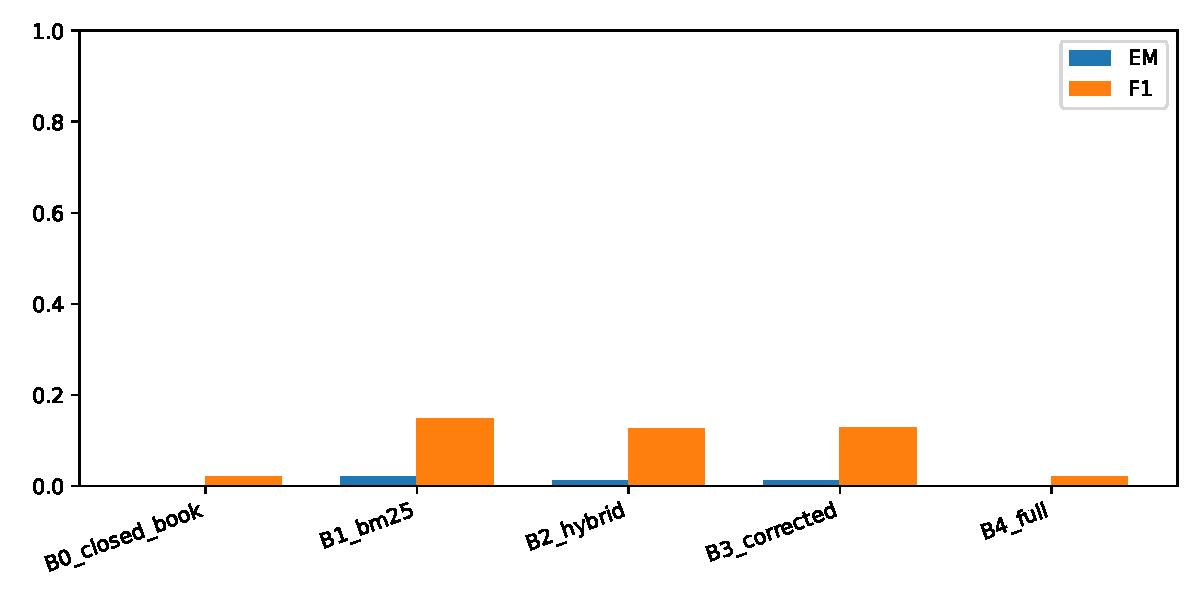
\includegraphics[width=.47\textwidth]{../results/plots/quality.pdf}\caption{Locked-test quality. Values derive from stored predictions.}\end{figure}
\clearpage
\section{Related Work}RAG combines parametric generation and non-parametric memory \cite{lewis2020rag}; DPR learns dense retrieval \cite{karpukhin2020dpr}. Self-RAG introduces reflection tokens and adaptive retrieval \cite{asai2024selfrag}, while corrective RAG evaluates retrieval quality before corrective actions \cite{yan2024crag}. Our policy differs by using transparent lexical features, a fixed single feedback round, and separately fitted correctness calibration. Classical calibration work warns that raw scores need not be probabilities \cite{guo2017calibration}; selective classification formalizes risk under abstention \cite{geifman2017selective}.
\section{Architecture}Let sparse and LSI ranks be $r_s(d)$ and $r_l(d)$. Reciprocal-rank fusion scores $R(d)=(60+r_s)^{-1}+(60+r_l)^{-1}$. The highest-overlap sentence produces an extractive candidate. Logistic regression returns proxy support $s$. If $s<0.62$, new evidence terms expand the query, the selected chunk is excluded, and retrieval runs once more. A second logistic model maps features and $s$ to $\hat p=P(\mathrm{EM}=1\mid x)$. The answer is emitted only when $\hat p\ge\tau$.
\begin{table}[b]\centering\caption{Component provenance}\scriptsize\begin{tabular}{lll}\toprule Component&Provenance&Role\\\midrule TF--IDF/LSI&project fit, scikit-learn&retrieval\\Verifier&project-trained logistic&support proxy\\Generator&project code&extractive candidate\\Calibrator&project-trained logistic&EM probability\\\bottomrule\end{tabular}\end{table}
\clearpage
\section{Training and Data}SQuAD 2.0 \cite{rajpurkar2018know} was downloaded from its official repository (SHA-256 recorded). Positives are sentences containing an annotated answer; weak negatives are same-passage sentences lacking every annotated answer string. Thus the task is answer-bearing evidence detection, not entailment. Article grouping separates 520 training and 164 held-out pairs. A dedicated 100-question split fits the correctness calibrator, another 100 selects $\tau$, and 150 questions form the locked test. Fifty separate tests remove the annotated source document; this establishes controlled unavailability, not global unanswerability.
\section{Protocol}B0 is closed-book abstention; B1 uses lexical retrieval; B2 adds LSI fusion; B3 adds proxy verification and correction; B4 adds calibration and abstention. All baselines use identical IDs. EM and token F1 use normalized multiple-gold matching. Retrieval recall checks whether the annotated passage appears in top five. Ten equal-width bins produce ECE; Brier score targets EM. Risk is $1-\mathrm{accuracy}$ among answered items and coverage is the answered fraction. One thousand question-level bootstrap resamples produce percentile intervals.
\begin{figure}[b]\centering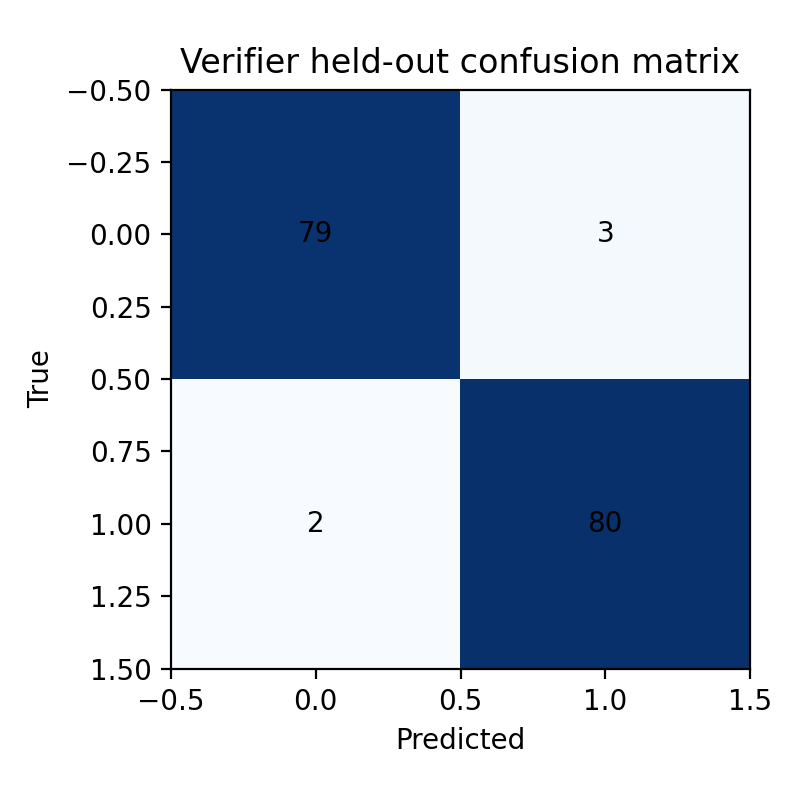
\includegraphics[width=.42\textwidth]{../results/plots/verifier_confusion.png}\caption{Held-out verifier confusion matrix (answer-bearing proxy).}\end{figure}
\clearpage
\section{Results}Table~\ref{tab:main} reports the real pilot. BM25 had the best measured retrieval recall and quality. Hybrid fusion reduced recall by 0.087 and did not improve answer quality. Correction increased median latency from 1.59 to 3.47 ms but produced no EM gain. The verifier achieved 0.970 macro-F1 versus a 0.500 majority baseline, mainly because answer-substring features closely match its proxy label.
\begin{table}[t]\centering\caption{Locked test, $n=150$}\label{tab:main}\scriptsize\begin{tabular}{lrrrr}\toprule Method&EM&F1&Recall@5&Coverage\\\midrule B0&.000&.020&.000&.000\\B1&.020&.148&.587&1.000\\B2&.013&.126&.500&1.000\\B3&.013&.130&.513&1.000\\B4&.000&.020&.513&.000\\\bottomrule\end{tabular}\end{table}
\section{Calibration and Selectivity}For B4, ECE was 0.195 and Brier score 0.049. The validation-selected threshold targeting risk at most 0.20 answered no test items, so test selective risk is undefined rather than zero. AURC was 0.993. All 50 source-withholding cases were also abstained on. This behavior avoids unsupported output but has no practical utility at zero coverage.
\begin{figure}[b]\centering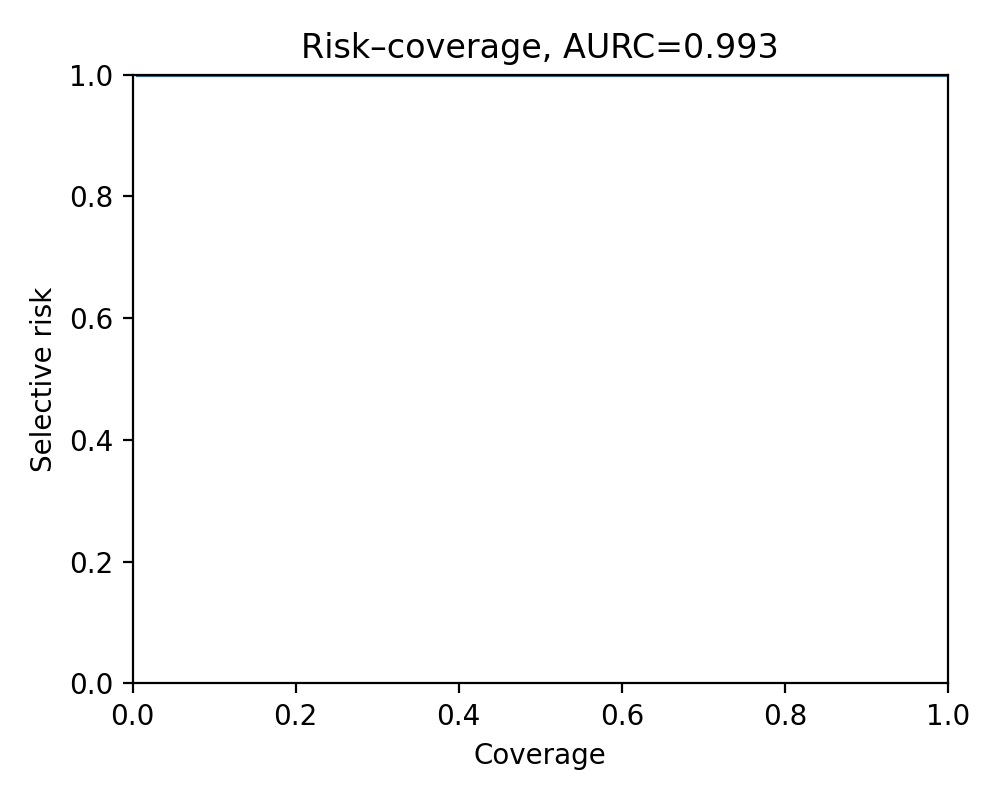
\includegraphics[width=.46\textwidth]{../results/plots/risk_coverage.png}\caption{Risk--coverage curve; lower is better.}\end{figure}
\clearpage
\section{Ablation and Resource Analysis}B2 versus B1 isolates fusion; B3 versus B2 adds correction; B4 versus B3 adds calibration and abstention. The comparison shows no quality gain from fusion or correction. Median latency was 1.47 ms (B1), 1.59 ms (B2), 3.47 ms (B3), and 3.55 ms (B4), excluding one-time index fitting. B3 averaged 1.8 retrieval and candidate-generation calls. The run used three Linux vCPUs and 9.7 GiB available RAM. Peak process RAM was not instrumented and is pending; no value is fabricated.
\section{Threats to Validity}The extractive rules are weak, and exact match penalizes semantically correct longer strings. Proxy support rewards literal answer occurrence and is not independent evidence that hallucination decreased. The sampled development questions and in-memory corpus limit generalization. Article overlap is audited, but late split top-up may introduce article overlap; question IDs remain disjoint. A single pipeline run and classifier seed cannot measure seed variance. There are no human judgments. Windows commands were authored but only Linux execution was observed.
\section{Failure Analysis}Correction often expands with terms from irrelevant evidence, reinforcing a bad retrieval neighborhood. LSI fusion underperformed lexical retrieval on this sample. Calibration saw few correct candidates and therefore selected a conservative threshold. These failures motivate a stronger local generator, semantic entailment labels, and threshold objectives that explicitly impose minimum coverage.
\clearpage
\section{Discussion}RQ1 is answered negatively for this pilot: correction did not improve EM or F1. RQ2 is inconclusive: calibration produced a low Brier score largely because positives were rare, while ECE remained 0.195. RQ3 shows reduced emitted error only by collapsing coverage to zero, which is not useful. RQ4 indicates lexical retrieval was the strongest implemented retrieval variant and that generation quality is the binding constraint.
\section{Reproducibility and Ethics}Every prediction, citation, correction query, and latency is stored. Plots regenerate from JSONL. The dashboard performs live local inference. Dataset provenance and licenses are recorded. The system must not be used for medical, legal, or other high-stakes answers. The annotation template proposes two independent student annotators and one adjudicator, but results remain pending.
\section{Conclusion}We built and executed an evidence-calibrated, bounded-correction RAG pipeline on CPU, trained two local components, and exposed a useful negative result: calibration cannot rescue a generator that is almost always wrong. The system's abstention is honest but overly conservative. Future work should replace the heuristic generator, use genuine entailment supervision, preserve strict group splits, measure peak memory, and repeat training across seeds before making stronger claims.
\bibliographystyle{IEEEtran}\bibliography{references}
\end{document}

